%%%%%%%%%%%%%%%%%%%%%%%%%%%%%%%%%%%%%%%%%%%%%%%%%%%%%%%%%%%%%%%%%%%%%%%%%
%
% This file defines the style for your homebook
% You don't need to edit it any more, if not to 
% change the authors name:
%
% Search below for the keyword:   GROUP
% insert your group number
%
% Search below for the keyword:   AUTHORS
% insert the name of the authors
%
%%%%%%
% Now to update the dexcription  of your work you will 
% use the file ``master.tex'' in the current directory
% following the instructions in it 
%
%%%%%% 
%%%%%%  
%%%%%%
% If you want to compile your document you have TWO ways
% depending on the fact that 
% 	1) you have inserted only postcript images in your tex file 
%		---> then go to MODE 1
%	2) you have inserted other kind of images (jpg..) in your tec file
%		---> then go to MODE 2
%
% MODE 1 
%simple type:
% 	latex homebook.tex
%
% If the compilation runs succesfully and you want to see the results type:
% 	xdvi homebook.dvi &
% and use the menus to go through the document
%
% If you want to create a pdf type:
% 	dvipdfm homebook.dvi
%
% a homebook.pdf file is created
% you can see it using the command:
% 	acroread homebook.pdf &
%
%
% MODE 2
% simple type:
%	pdflatex homebook.tex
%
% If the compilation runs succesfully you directly have the pdf file
% and you can see it using the command:
%       acroread homebook.pdf &
%
% 
%%%%%%%%%%%%%%%%%%%%%%%%%%%%%%%%%%%%%%%%%%%%%%%%%%%%%%%%%%%%%%%%%%%%%%%%%%
\documentclass[10pt,  english, makeidx, a4paper, titlepage, oneside]{book}
\usepackage{babel}
\usepackage{fancyhdr}
\usepackage{makeidx}
\usepackage{titlesec}
\usepackage{listings}
\usepackage{xcolor} 
\usepackage{booktabs}
\usepackage{multirow}
\usepackage{graphicx}

\definecolor{mGreen}{rgb}{0,0.6,0}
\definecolor{mGray}{rgb}{0.5,0.5,0.5}
\definecolor{mPurple}{rgb}{0.58,0,0.82}
\definecolor{backgroundColour}{rgb}{0.95,0.95,0.92}

\lstdefinestyle{CStyle}{
    backgroundcolor=\color{backgroundColour},   
    commentstyle=\color{mGreen},
    keywordstyle=\color{magenta},
    numberstyle=\tiny\color{mGray},
    stringstyle=\color{mPurple},
    basicstyle=\footnotesize,
    breakatwhitespace=false,         
    breaklines=true,                 
    captionpos=b,                    
    keepspaces=true,                 
    numbers=left,                    
    numbersep=5pt,                  
    showspaces=false,                
    showstringspaces=false,
    showtabs=false,                  
    tabsize=2,
    language=C
}

\newenvironment{listato}{\footnotesize}
                        {\normalsize }


%\pagestyle{empty}

\textwidth 15.5cm
\textheight 23cm
\topmargin -1cm
\oddsidemargin -0.0cm
\linespread{1.1}

\pagestyle{fancy}
\lhead{}
\chead{GPU programming}
\lfoot{}
\cfoot{}
\rfoot{}
\rhead{\thepage}

\usepackage{graphicx}
\usepackage{amsmath}
\usepackage{amsfonts}
\usepackage{amsthm}
\usepackage{amssymb}
\usepackage{tabularx}
\usepackage{hyperref}
\usepackage{caption}
\usepackage{subcaption}
\usepackage[mediumspace,mediumqspace,Grey,squaren]{SIunits}
%\oddsidemargin -1.1cm

\titleformat{\chapter}[display]
{\normalfont\Large\filcenter\sffamily}
{\titlerule[0.5pt]%
\vspace{1pt}
\titlerule
\vspace{1pc}
\LARGE\MakeUppercase{\chaptertitlename} \thechapter
}
{1pc}
{\titlerule
\vspace{1pc}
\Huge}

\newcommand{\SubSubSection}[1]{\subsubsection{\bf Exercise   ~#1}}

\newcommand{\homework}[1]{\subsubsection{\bf Homework   ~#1}}

\newcommand{\Solution}{\subsubsection{\bf Solution}}




\makeindex
\begin{document}
\frontmatter
\begin{titlepage}
\vspace{2cm}
\centerline{

\includegraphics[width=2.5cm]{./logopoli.png}}  
\centerline{\LARGE Politecnico di Torino}
\bigskip
\centerline{\Large III Facolt\`a di Ingegneria}
\vspace{4cm}
\centerline{\Huge\sf Final project}
\bigskip
\centerline{\Huge\bfseries\sf Parallel high level synthesis using GPU}
\vspace{2cm}
\centerline{\LARGE Master degree in Software Engineering}
\vspace{4.4cm}
%%%%%%%%%%%%%%%%%%%%%%%%%%%%%%%%%%%%%%%%%%%%%%%%%%%%%%%
% GROUP
% Change the name of your group below
%
\centerline{\Large GPU programming}
\vspace{2cm}
%
%%%%%%%%%%%%%%%%%%%%%%%%%%%%%%%%%%%%%%%%%%%%%%%%%%%%%%%
% AUTHORS
% Change the name of the Group participants here
%
\centerline{Dilillo Nicola S284963}
%
%%%%%%%%%%%%%%%%%%%%%%%%%%%%%%%%%%%%%%%%%%%%%%%%%%%%%%
\vspace{2cm}
\centerline{\href{https://github.com/nicoladilillo/GPU_final_project}{GitHub Repository}}
\vspace{1cm}
%{\scriptsize Many thanks to Prof. Mariagrazia Graziano for providing us with this template.}
\end{titlepage}

\tableofcontents

%%%%%%%%%%%%%%%%%%%%%%%%%%%
% 
\mainmatter
\lstset{language=VHDL}

%%%%%%%%%%%%%%%%%%%%%%%%%%%%%%%%%%%%%%%%%%%%%%%%%%%%%%
%    
% HERE IS WHERE YOU INCLUDE YOUR CHAPTERS
%
%%%%%%%%%%%%%%%%%%%%%%%%%%%%%%%%%%%%%%%%%%%%%%%%%%%%
% This will help you in writing your homebook
% Remember that the character % is a comment in latex
%
% chapter 1
\chapter{Introduction}
\label{chap1}

\section{Motivation}
A lot of EDA tools used a heuristic approaches to solve synthesis for electronic circuits. In high level synthesis (HLS) there could be two types of constrained: area or time. Exact algorithms are not use to solve those kinds of problems because solutions will occur after a lot of time, even years. In this project the main purpose is to exploit the parallelism of the GPU to create all the possible set of combination of resources, that satisfy area constrain, and through the usage of a list scheduling algorithm evaluate which is the fastest among all.

To evaluate all the benefits of GPU algorithm version a CPU one has been written. The basic concept is the same but in the latter a the classical sequential approach has been used.

\section{Terms clarification}

Before to move on a little refresh about general topic of this project is mandatory.

Synthesis is the process that generate the circuit netlist of a certain circuit model, given a set of library and a target device. High level synthesis (HLS), also known as behavioral synthesis and algorithmic synthesis, is a design process in which a high level functional description of a design is automatically compiled into a RTL implementation that meets certain user specified design constraints. 

Topically HLS is divided in three main phase:

\begin{itemize}
    \item Allocation, choice of how many resources will be used;
    \item Scheduling, of the processes on the set of selected resources;
    \item Binding of operations to resources.
\end{itemize}{}

Simultaneous solution of these three problems would lead to better results (closer to the Pareto-optimal set), but it is typically too complex.
A Pareto point is a solution that is better than the other under certain aspect and is not dominated by any other.

\subsection{List scheduling}
\label{list_scheduling}

List scheduling is a greedy algorithm that takes as inputs a list of jobs that should be executed on a set of resources, that is also given. The list is ordered according a priority criteria, that could be not always the same. The algorithm repeatedly executes the following steps until a valid schedule is obtained:
\begin{itemize}
    \item Take the first job in the list (the one with the highest priority).
    \item Find a resources that is available for executing this job.
    \item If a resources is found, schedule this job on it, otherwise (no suitable machine is available), select the next job in the list.
    \item Repeat until resources are not more available or there are not node to schedule.
\end{itemize}

To obtain a valid schedule all nodes have to been scheduled in a finite time respected the resources number constraints.

\subsection{Example}
Let's try to synthesis the following function $F = a*b + a*c$, that is represented by the DFG in figure \ref{fig:DFG}. It's important to note that each node of the DFG is binary, receive at most two inputs, and that each node will be assign to a specific resources in a given instant of time.

\begin{figure}[h]
\centering
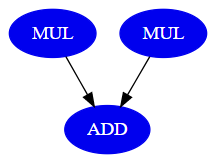
\includegraphics[height=5cm\textwidth]{report_template/chapters/figures/dfg.png}
\caption{DFG of $F = a*b + a*c$}
\label{fig:DFG}
\end{figure}

Two possible schedules could be picked, like shows in figure \ref{fig:DFG_schedules}. Both are Pareto-optimal but in the left one just two resources have been used (one adder and one multiplier) while in the right one is present a further multiplier. Of curse the latter has littler latency.
 
\begin{figure}[h]
\centering
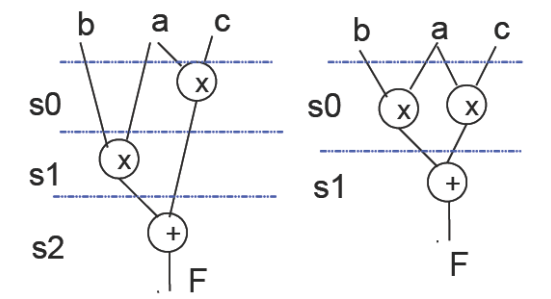
\includegraphics[height=5cm\textwidth]{report_template/chapters/figures/dfg_scheduled.png}
\caption{On the left there is a bigger latency but less resources are used, while on the right a littler latency occur but more resource are used.}
\label{fig:DFG_schedules}
\end{figure}

The purpose of this project is to select the set of resources that allows to have the lowest latency and that respect a certain value of area constraint.
In this case let's suppose that each resources has an unitary value of area and the limit is 2,  the first schedules will be the one chosen.

The following schedules is then convert in hardware, like shows in figure \ref{fig:HW_schedules}.

\begin{figure}[h]
\centering
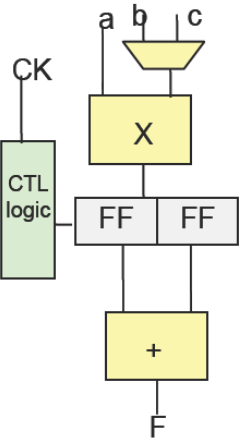
\includegraphics[height=6cm\textwidth]{report_template/chapters/figures/HW_scheduling.png}
\caption{Hardware implementation}
\label{fig:HW_schedules}
\end{figure}

\section{How to proceed}

The synthesis tools used to schedule DFG through the usage of efficient heuristic solutions that find optimal solutions because those approaches are not exhaustive and don't use exact scheduling algorithm (like ILP). 

The purpose of this project is to explore all the set of resources combinations and, based on a list scheduling algorithm, choose which one retrieve the smallest latency. In order to do that GPU is exploited to create all those combinations in parallel and for each calculate the schedule time using the same criteria.

As first attempt a sequential version, runnable on CPU, has been written and different versions for GPU, in order too see which one will be the fastest.

All the available DFGs used for test have been taken from another course and for this project purpose the format has been a little modify, through a python algorithm, to have a faster computation in cuda language. The original one are available and usable to retrieve a visual interpretation of operations.









\chapter{Parallelization}
\label{chap2}

The advantage of GPU implementation derive to the possibility to create all possible combinations of resources in a parallel way and not sequentially. Theoretically this means that in a single instant the entire set is created, practically little amount of time pass between one and other.

\section{Combination}

Formula \ref{comb_formula} indicates all to possible combinations that can be extract from a set of n elements choosing group of k elements. In this case the n indicate the occurrence of resources. 

\begin{equation}
    \binom{n}{k} = \frac{n!}{k!(n-k)!}
    \label{comb_formula}
\end{equation}

The complete power set to formulate has an occurrence equal to the sum of all combination from the minimal number of resources needed to the max number, like show in formula \ref{power_set}.

\begin{equation}
    \sum_{i=k_{min}}^{k_{max}} \binom{n}{i} = 
    \sum_{i=k_{min}}^{k_{max}} \frac{n!}{i!(n-i)!}
    \label{power_set}
\end{equation}

\section{Combinadic}

Combinadic is a useful technique that, giving and index in the range between 0 and $\binom{n}{k}-1$ , return a unique combination set of k element, produced in lexicographic order.

From a given combination is possible to find the corresponding number $N$, corresponding to 
$c_k > ... > c_2 > c_1$, according formula \ref{id_Combinadic}.
 
\begin{equation}
    N = \binom{c_k}{k} + ... + \binom{c_2}{2} + \binom{c_1}{1}
    \label{id_Combinadic}
\end{equation}

From number $N$ is more diffucult extract the combination. By the definition of the lexicographic ordering, two k-combinations that 
differ in their largest element ck will be ordered according to the comparison of those largest elements, from which it follows that all
combinations with a fixed value of their largest element are contiguous in the list. Moreover the smallest combination with ck as
the largest element is $\binom {c_{k}}{k}$, and it has $c_i = i - 1$ for all $i < k$ (for this combination all terms 
in the expression except $\binom {c_{k}}{k}$ are zero). 

Therefore $c_k$ is the largest number such that $\binom {c_{k}}{k} \leq N$. 
If $k > 1$ the remaining elements of the k-combination form the (k-1)-combination corresponding to the number
$N - \binom {c_{k}}{k}$ in the combinatorial number system of degree k - 1, and can therefore be found 
by continuing in the same way for $N - \binom {c_{k}}{k}$ and k - 1 instead of N and k.

\subsection{Example}

Suppose one wants to determine the 5-combination at position 72.
The successive values of $\binom {n}{5}$ for n = 4, 5, 6, ... are 0, 1, 6, 21, 56, 126, 252, ..., of which the largest 
one not exceeding 72 is 56, for n = 8. Therefore c5 = 8, and the remaining elements form the 4-combination at position 
72 - 56 = 16. The successive values of $\binom {n}{4}$ for n = 3, 4, 5, ... are 0, 1, 5, 15, 35, ..., of which the largest
one not exceeding 16 is 15, for n = 6, so c4 = 6. Continuing similarly to search for a 3-combination at position 16 1 15 = 1
one finds c3 = 3, which uses up the final unit.
This establishes $72=\binom{8}{5}+\binom{6}{4}+\binom {3}{3}$, and the remaining values $c_i$ will be the maximal ones with
$\binom{c_i}{i}=0$, namely $c_i = i - 1$. Thus we have found the 5-combination \{8, 6, 3, 1, 0\}.

\subsection{Combinadic in GPU}

Exploit Combinadic in GPU is pretty immediate. Each thread in GPU has an unique id value that goes from zero to the number of initialize thread minus one. 
This id could be used to take a specific combination where each element correspond to an id of a specific resource. 


\section{Repetition}

What explain until now is based on combination with no repetition but a resource can be instantiate more than once!

In a sequential algorithm the max repetition constraint is implemented since the beginning in the code while here it is develop in the thread differently, with it's own implementation. In this case also the CPU algorithm follow the same method in order to have a best prototype of the best parallel one.

Like will be show in the next chapter, will be not possible to create all repetitions of combinations set inside a single thread on the GPU, errors will arise due to time. To avoid this problem single thread should handle also each single repetition. In this way much more simple thread are created. While in the previous version all the repetition that respect area constraint are analyze and the useless are not created, now all ones are take into consideration.

To not explode computation a max of repetition for each resources is set.
\chapter{Implementation}
\label{chap3}

\section{CPU}

Before to proceed with the parallelization of this algorithm, a sequential version, executable on CPU, has been written. At the end the results will be the same and the only different will be the time of computation.

This is the prototype of final release, more easy to develop, especially for the final part that compare the best scheduling latency. Here big optimization are not so useful for better performance, used more or less memory not speed up the computation.

\section{GPU Data Structure}

To perform the GPU elaboration data structure has been changed in order to lighten the overall process of memory copy, the real bottleneck of this approach. For this reason the device has to shrink the data previous to pass them to host.

The main big information variables are related all about node and operation information. Both keep track of information that are not useful for scheduling computation and so, before to call GPU kernel, they are filtered to maintain only the main information.

To improve the elaboration also other variable are been accurately choose to use as less memory as possible.

\section{Scheduling Algorithm}

The section \ref{list_scheduling} explains which algorithm has been choose to performer scheduling operation. This part is identical both for GPU and CPU versions, change only the implementation of some variable, needed for final result, that correspond to a latency value. How will be explained in the next chapter those variables, to be more precise those arrays, will be the one of critical point that has to be improved to achieve better performance.


\section{GPU Kernel}

Different version has been created to see which will be the best approach to use to have the best performance.

By the way all of them use the same mechanism to analyze which repeated combination has the best latency. In the same block all threads save the result of latency and their own repeated combination on shared memory so, when all terminated the scheduling operation, the best set of resources is pick inside same block and pass to host trough the main memory. At the end CPU checks all combinations coming from kernel and choose the best one with minimum latency, in case of equality the one with minimum area is chosen. This part is implemented almost in the same way in all versions.

\subsection{Version 1}

The version one is base on the create thread that handle all repetition given a single combination. If not operation are covered the thread doesn't create the repetition. The single repetition scheduling is executed only if the area constraint is respected.

Combinations are group 1024 at a time, each using a single block inside a stream.

For long repetition time problems occurs and the kernel stops its execution.

\subsection{Version 2}

Each thread handle a single repeat combination and, also if the combination don't cover all the needed operation or if area constraint are not respected, the thread is created but the scheduling is not lunch. Different version has been created to test which is the best way to arrange variable declaration.

\begin{itemize}
    \item Version 2.0, like the previous one but with the new property of single repetition for thread.
    
    \item Version 2.1, use less shared memory that is compensated by dynamic allocation.
    
    \item Version 2.2, not use anymore dynamic allocation and improve the usage of resources, allocated a fix amount of memory.
    
    \item Version 2.3, instead of shared memory, arrays of fixed dimension are used inside each thread when possible and the global memory is called only when latency value obtain are better than before. Furthermore now, at the end execution of each blocks inside a thread, only thread with id zero take care to choose which has the best latency. 
\end{itemize}

From this version is pretty sure that dynamic allocation is a technique that needed a lot of time and not the best choice while, the usage of local register and call global memory as lest as possible, are big improvement.

Also here combinations are group 1024 at a time, each using a single block inside a stream.

\subsection{Version 3}

In previous version each stream handles single block while in this version each they are not more used and each kernel call works with all blocks that, given the combination $\binom{n}{k}$, has the same value of $k$. Now much more global memory is copy at the same time and this could result in an import speed up of the system.

\subsection{Version 4}

Merge the advantage of multi stream of version 2 and with the possibility to work with more blocks inside each stream of version 3. Then a further improved of version 4.1 has been add in order to have the possibility to have workload that stress the GPU with the creation of billion of threads.
\chapter{Results}
\label{chap4}

All tests, for CPU and GPU, had been run on the same device, Jetson Nano, the one provided from the course, and all 
results obtained are related to this hardware.

\section{Execution}

Before to run each execution be sure to compile using the available \emph{Makefile}.

To start execution it is possible run one of the bash scripts available.

\begin{itemize}
    \item \emph{run.sh}, to run all the GPU version.
    \item \emph{run\_CPU.sh}, to run all the CPU versions.
    \item \emph{run\_long.sh}, to run a long execution of a particular DFG using the version 4.1,
    the only that can carry such workload.
\end{itemize}

To run a single version directly three element are needed.

\begin{itemize}
    \item A file containing the DFG information, this file are obtained through original DFG file saved in .dot format.
    The conversion is achieved through a python script explained in appendix \ref{appendix1}.
    \item The value of area constrained.
    \item A file containing the all possible resources available. It is organized in the following way:
    \begin{itemize}
        \item first row is the number of operations k;
        \item then there are k rows containing the pair operation number and number n, representing the different resources;
        \item after each of these rows there are n row containing the pair area and speed of each resource that can execute that operation.
    \end{itemize}
\end{itemize}

The executable can be lunched in the following way:

\begin{lstlisting}
    dfg.o <dfg_name>.txt <RTL_file>.txt <area_constrained>
\end{lstlisting}

All latency, according DFG, are available inside a log file.

\section{Comparison}

In the following graphs, obtained from python script \emph{elaborate\_data.py} (appendix \ref{appendix2}),
it is possible to observe the performances of the all versions using different DFG and area constraint.
A lot of other tests had been run to check not only performances but also the correctness of the scheduling
but the ones show here are the most significant.
It's important to notice that version 1 is useless because, when it works, all versions, GPU and CPU,
have time execution almost equal to zero second.

\begin{figure}[!h]
    \centering
    \begin{subfigure}{.45\textwidth}
        \centering
        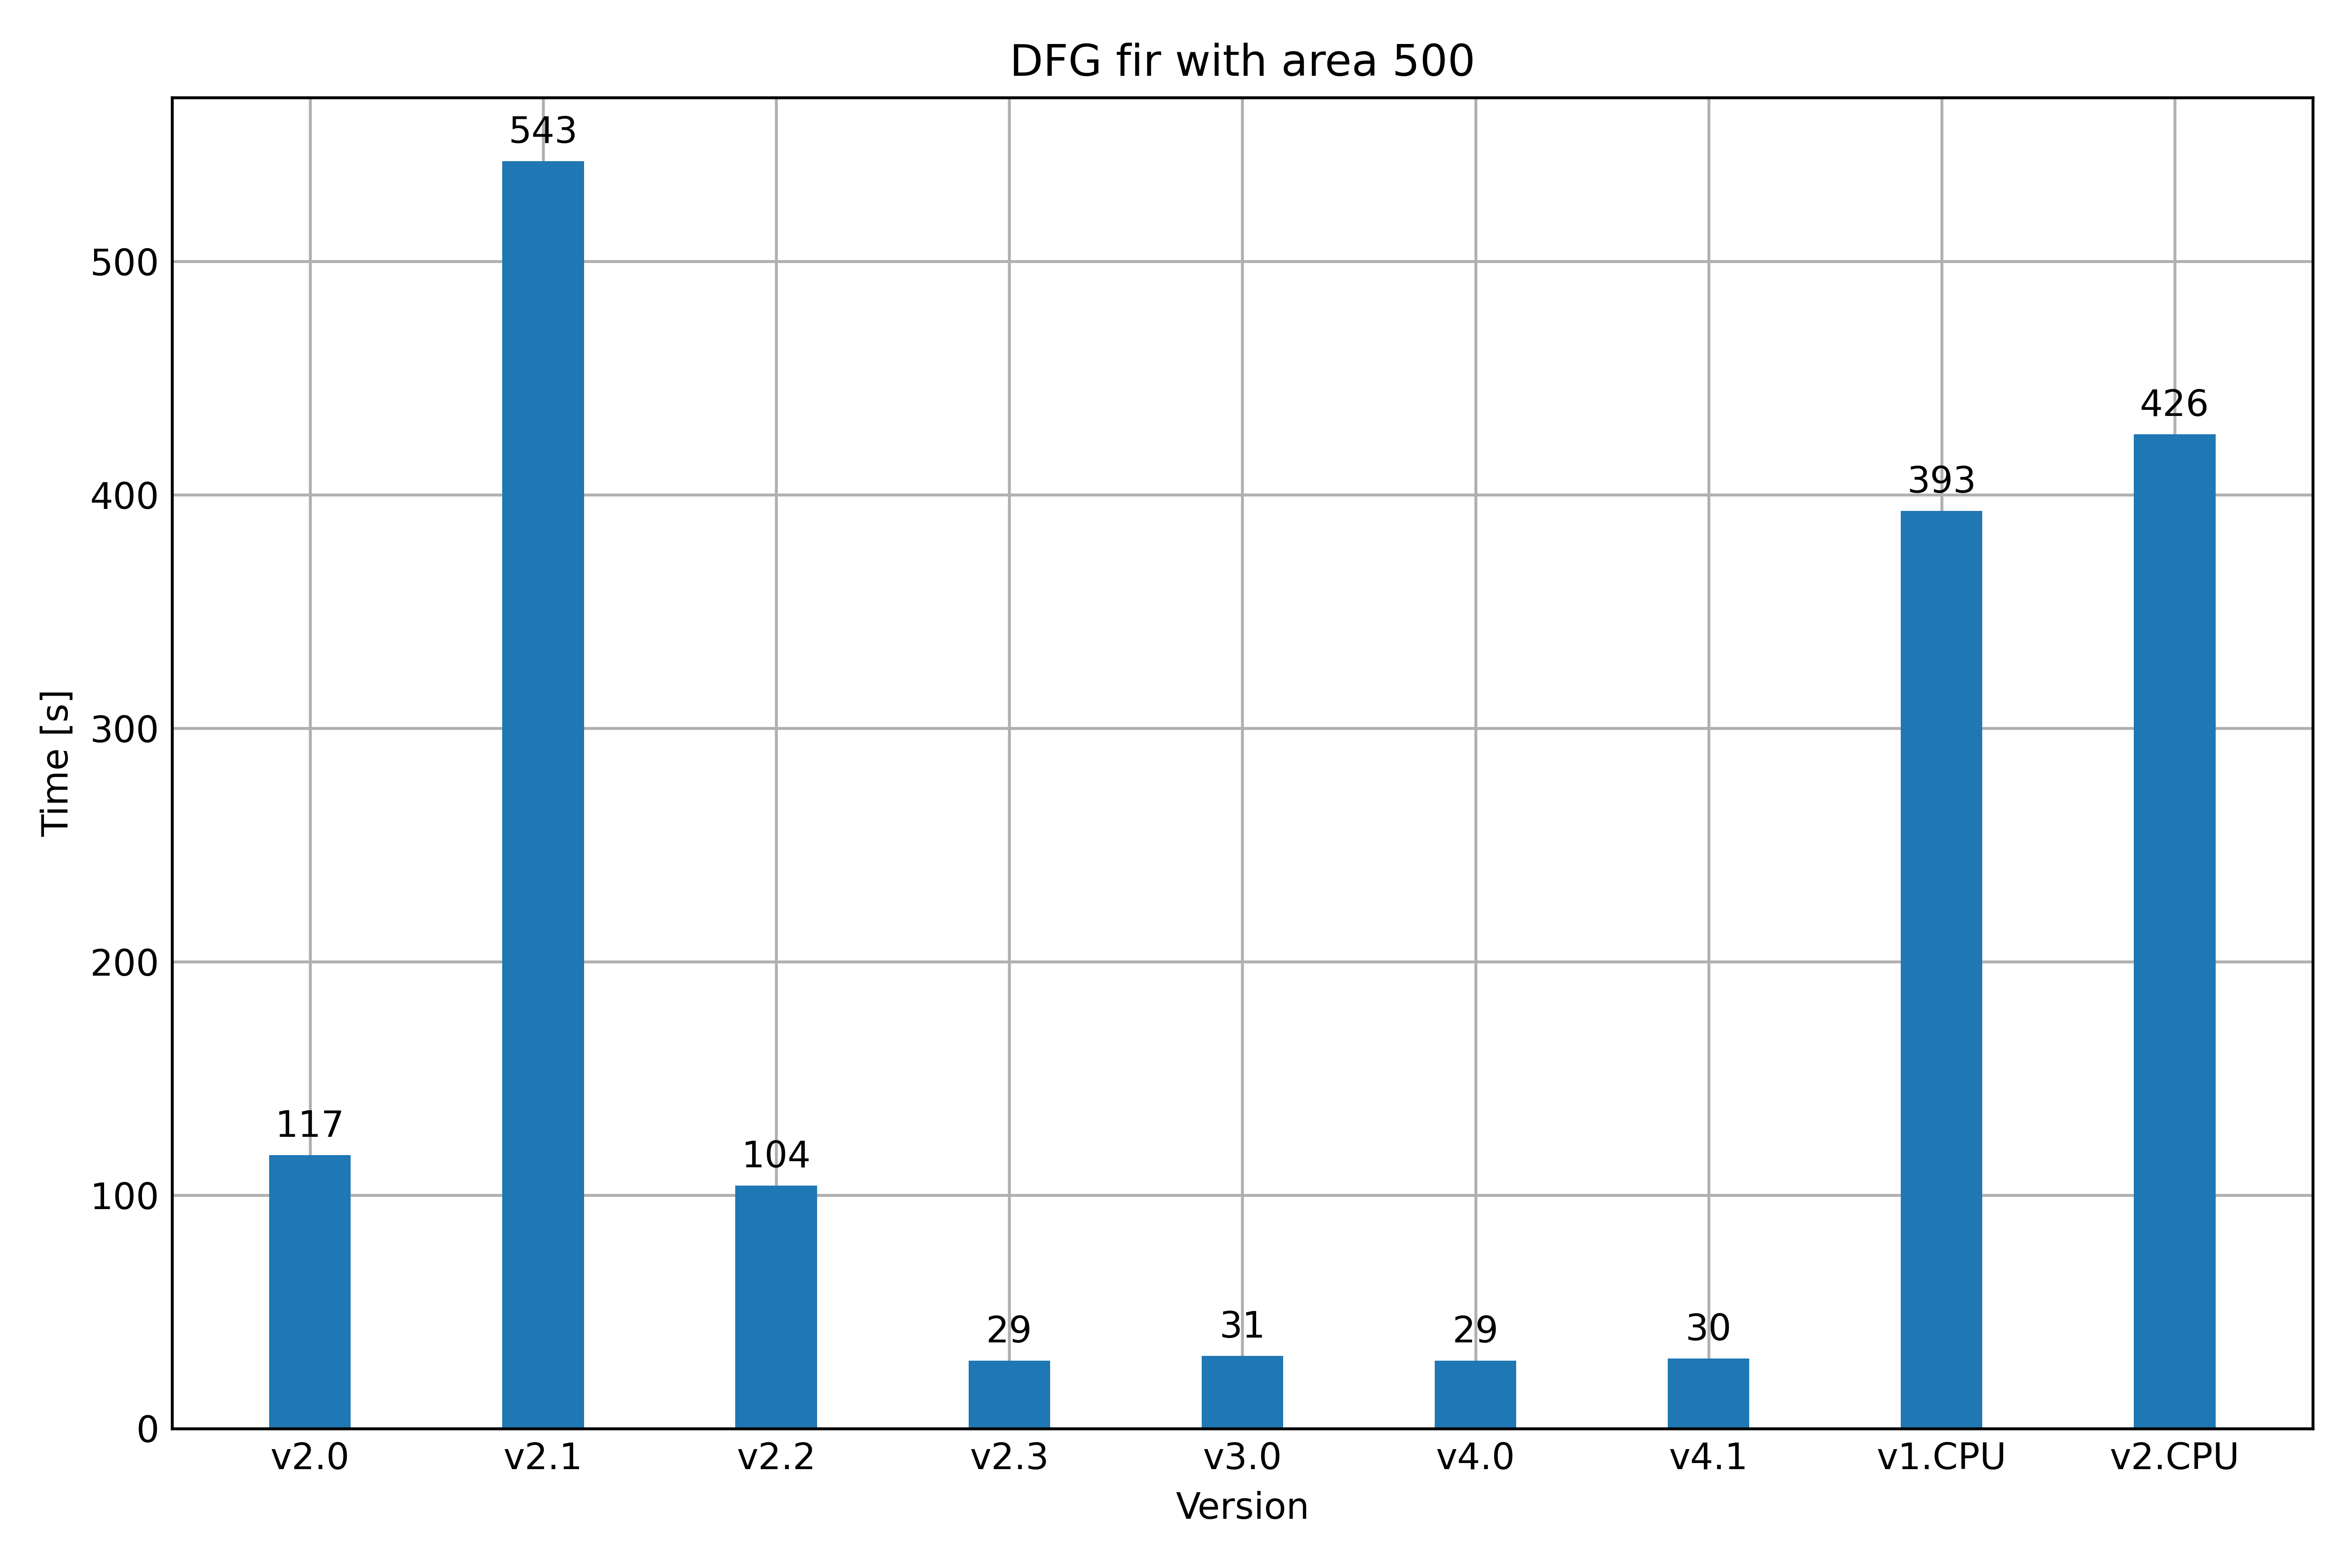
\includegraphics[width=.95\linewidth]{chapters/figures/fir_500.png}  
        \caption{fir bar graph with area 500}
        \label{fig:fir_500}
    \end{subfigure}
    \begin{subfigure}{.45\textwidth}
        \centering
        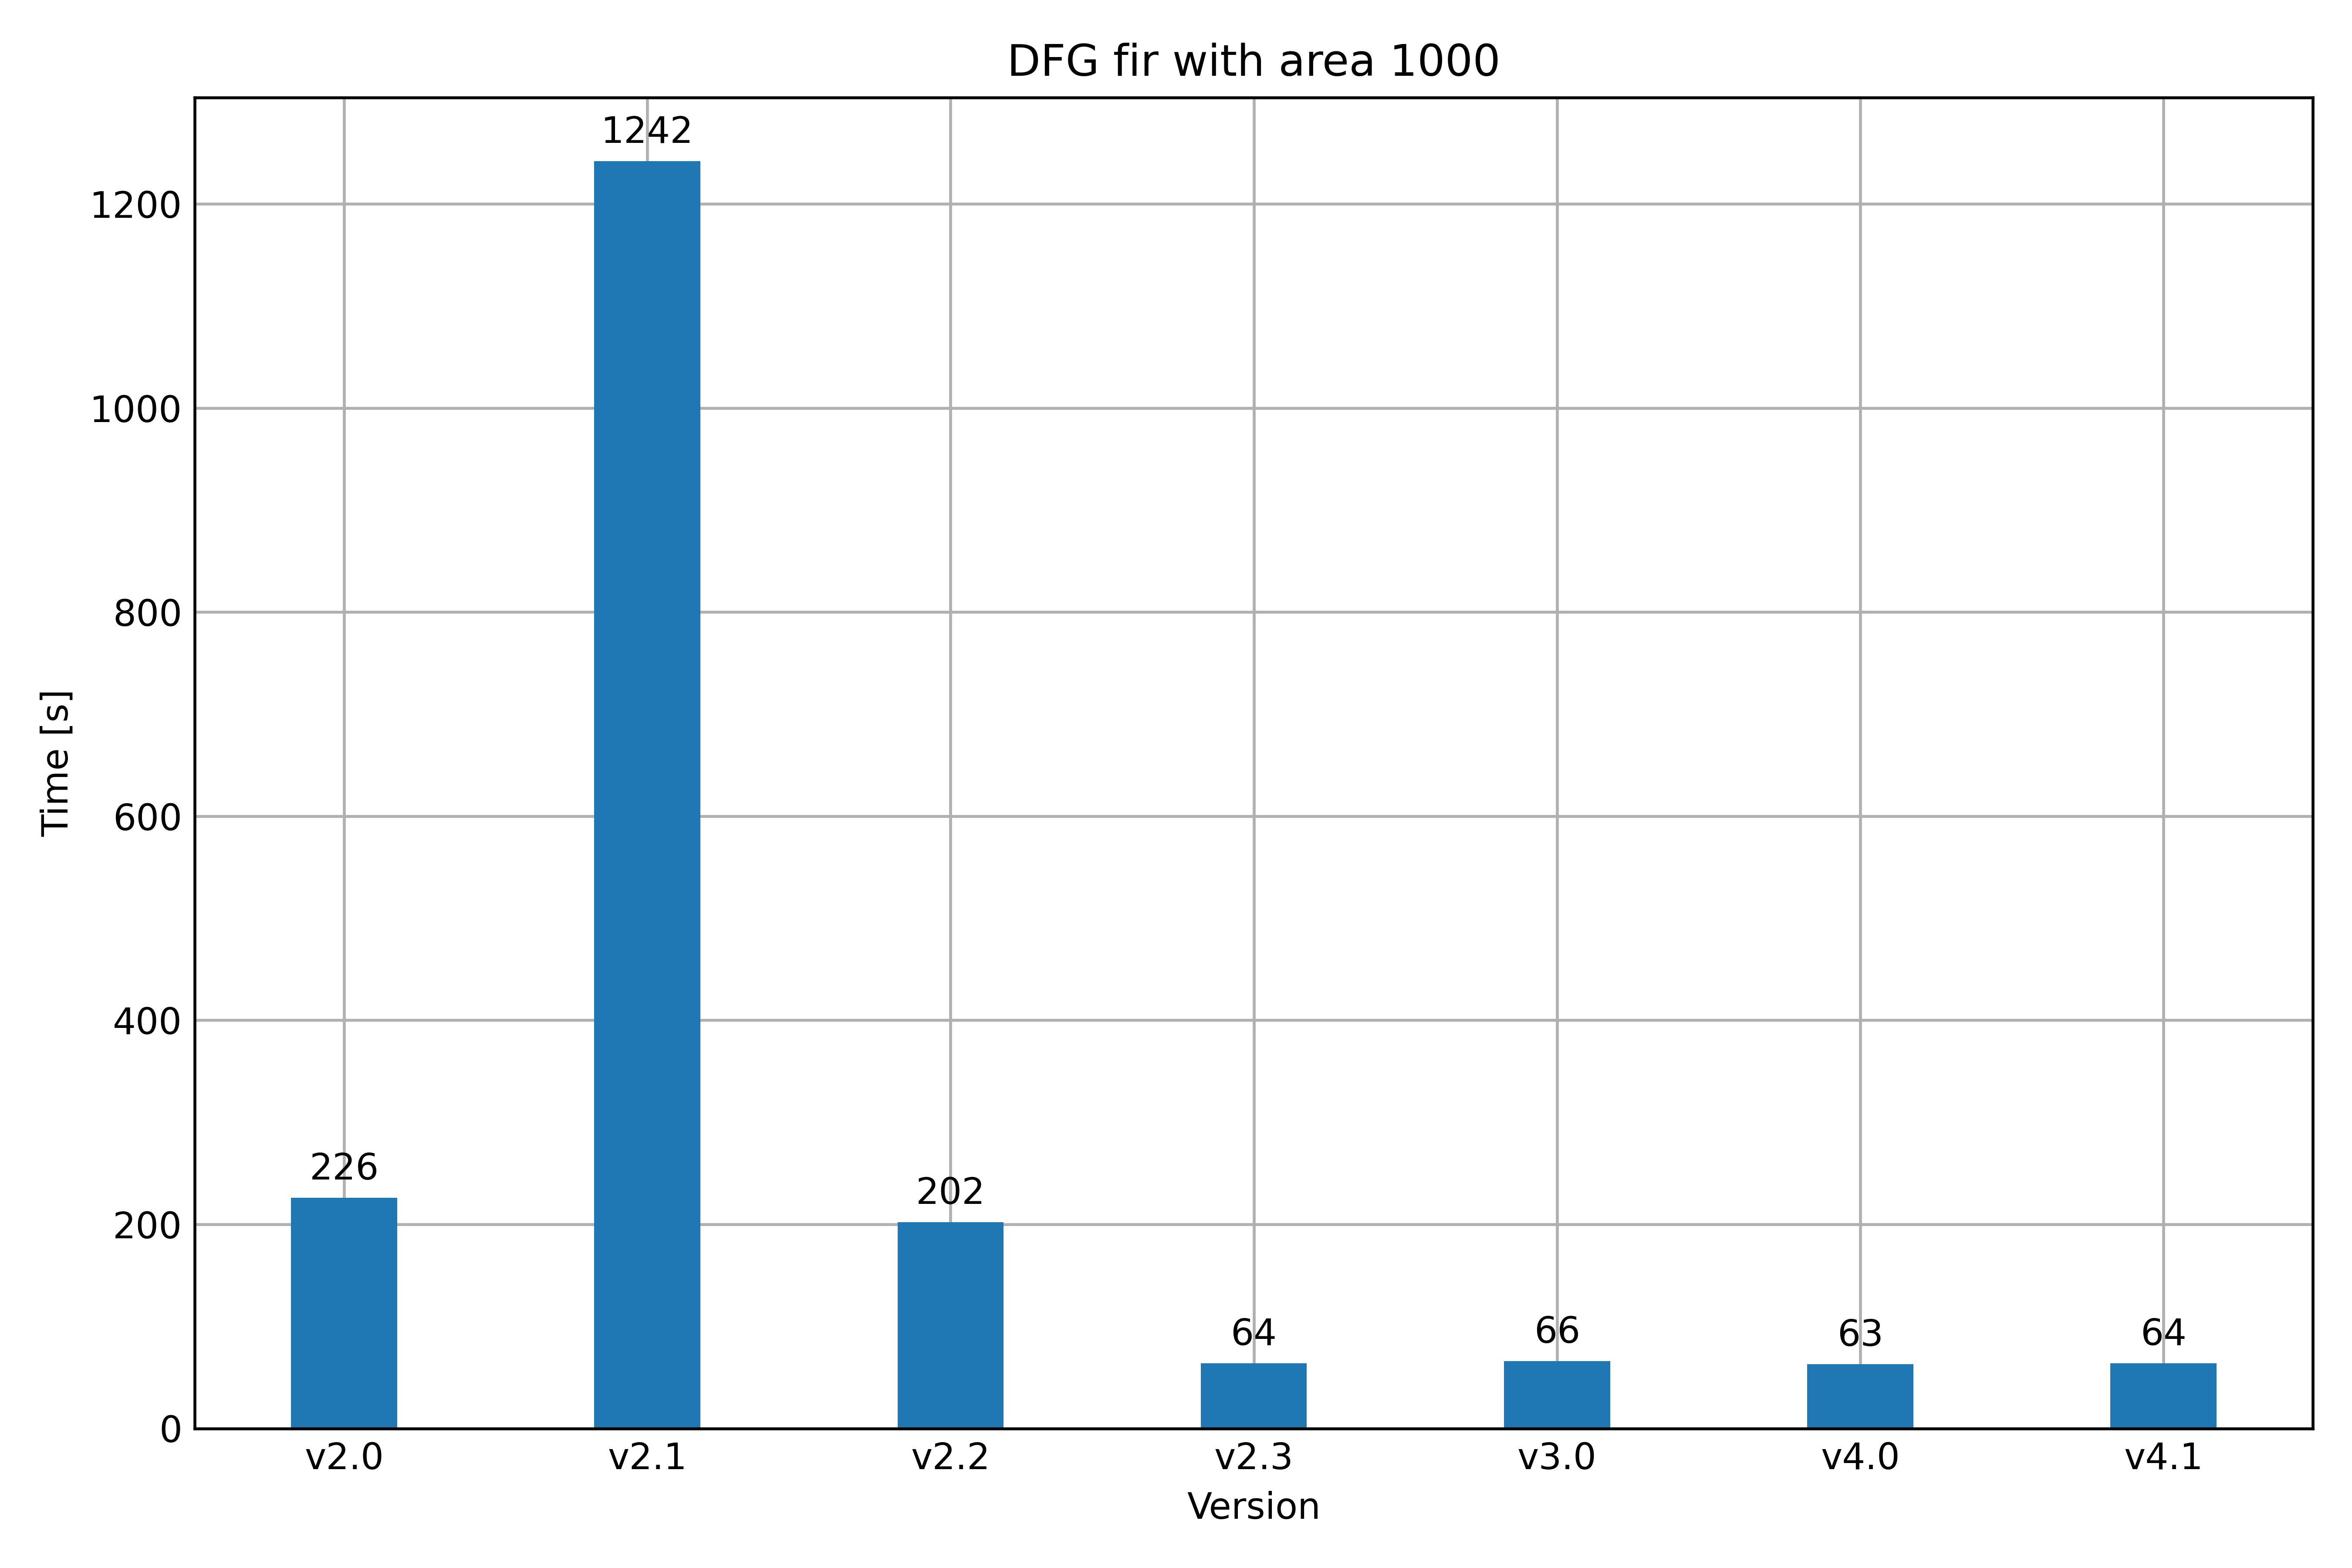
\includegraphics[width=.95\linewidth]{chapters/figures/fir_1000.png}  
        \caption{fir bar graph with area 1000}
        \label{fig:fir_1000}
    \end{subfigure}
\end{figure}

\begin{figure}[h]
    \centering
    \begin{subfigure}{.45\textwidth}
        \centering
        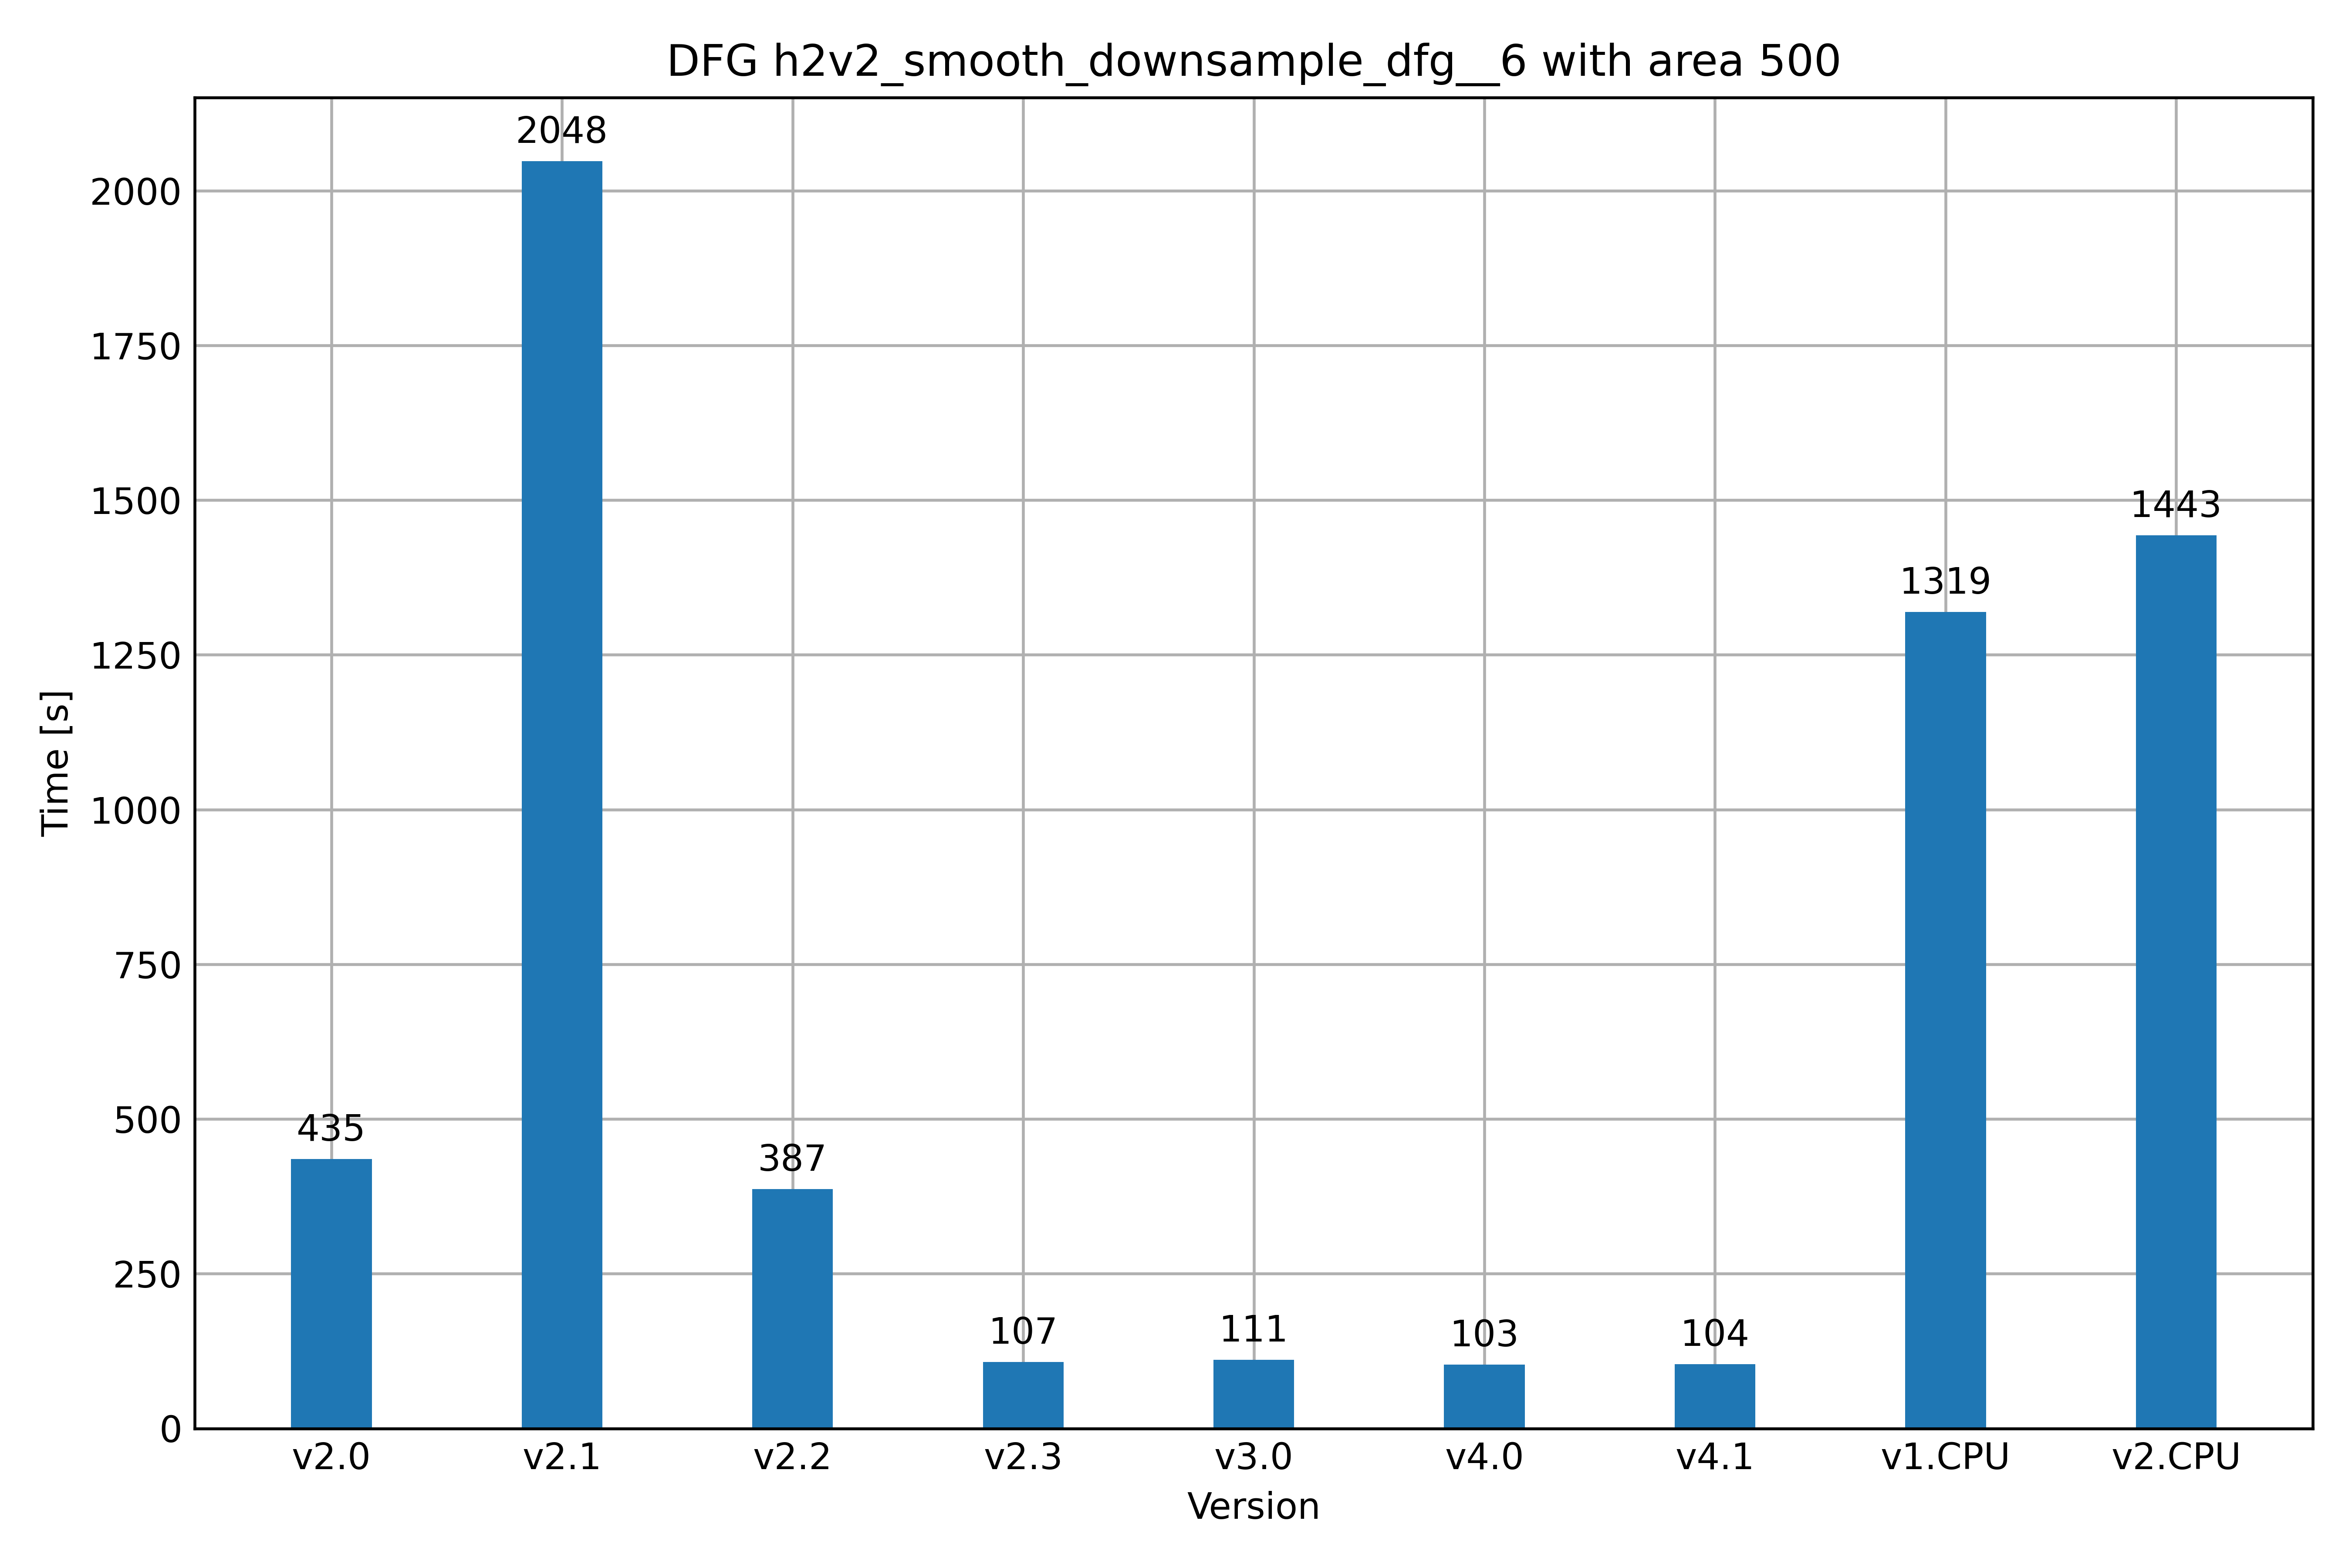
\includegraphics[width=.95\linewidth]{chapters/figures/h2v2_smooth_downsample_dfg__6_500.png}  
        \caption{h2v2 with area 500 bar graph}
        \label{fig:h2v2_500}
    \end{subfigure}
    \begin{subfigure}{.45\textwidth}
        \centering
        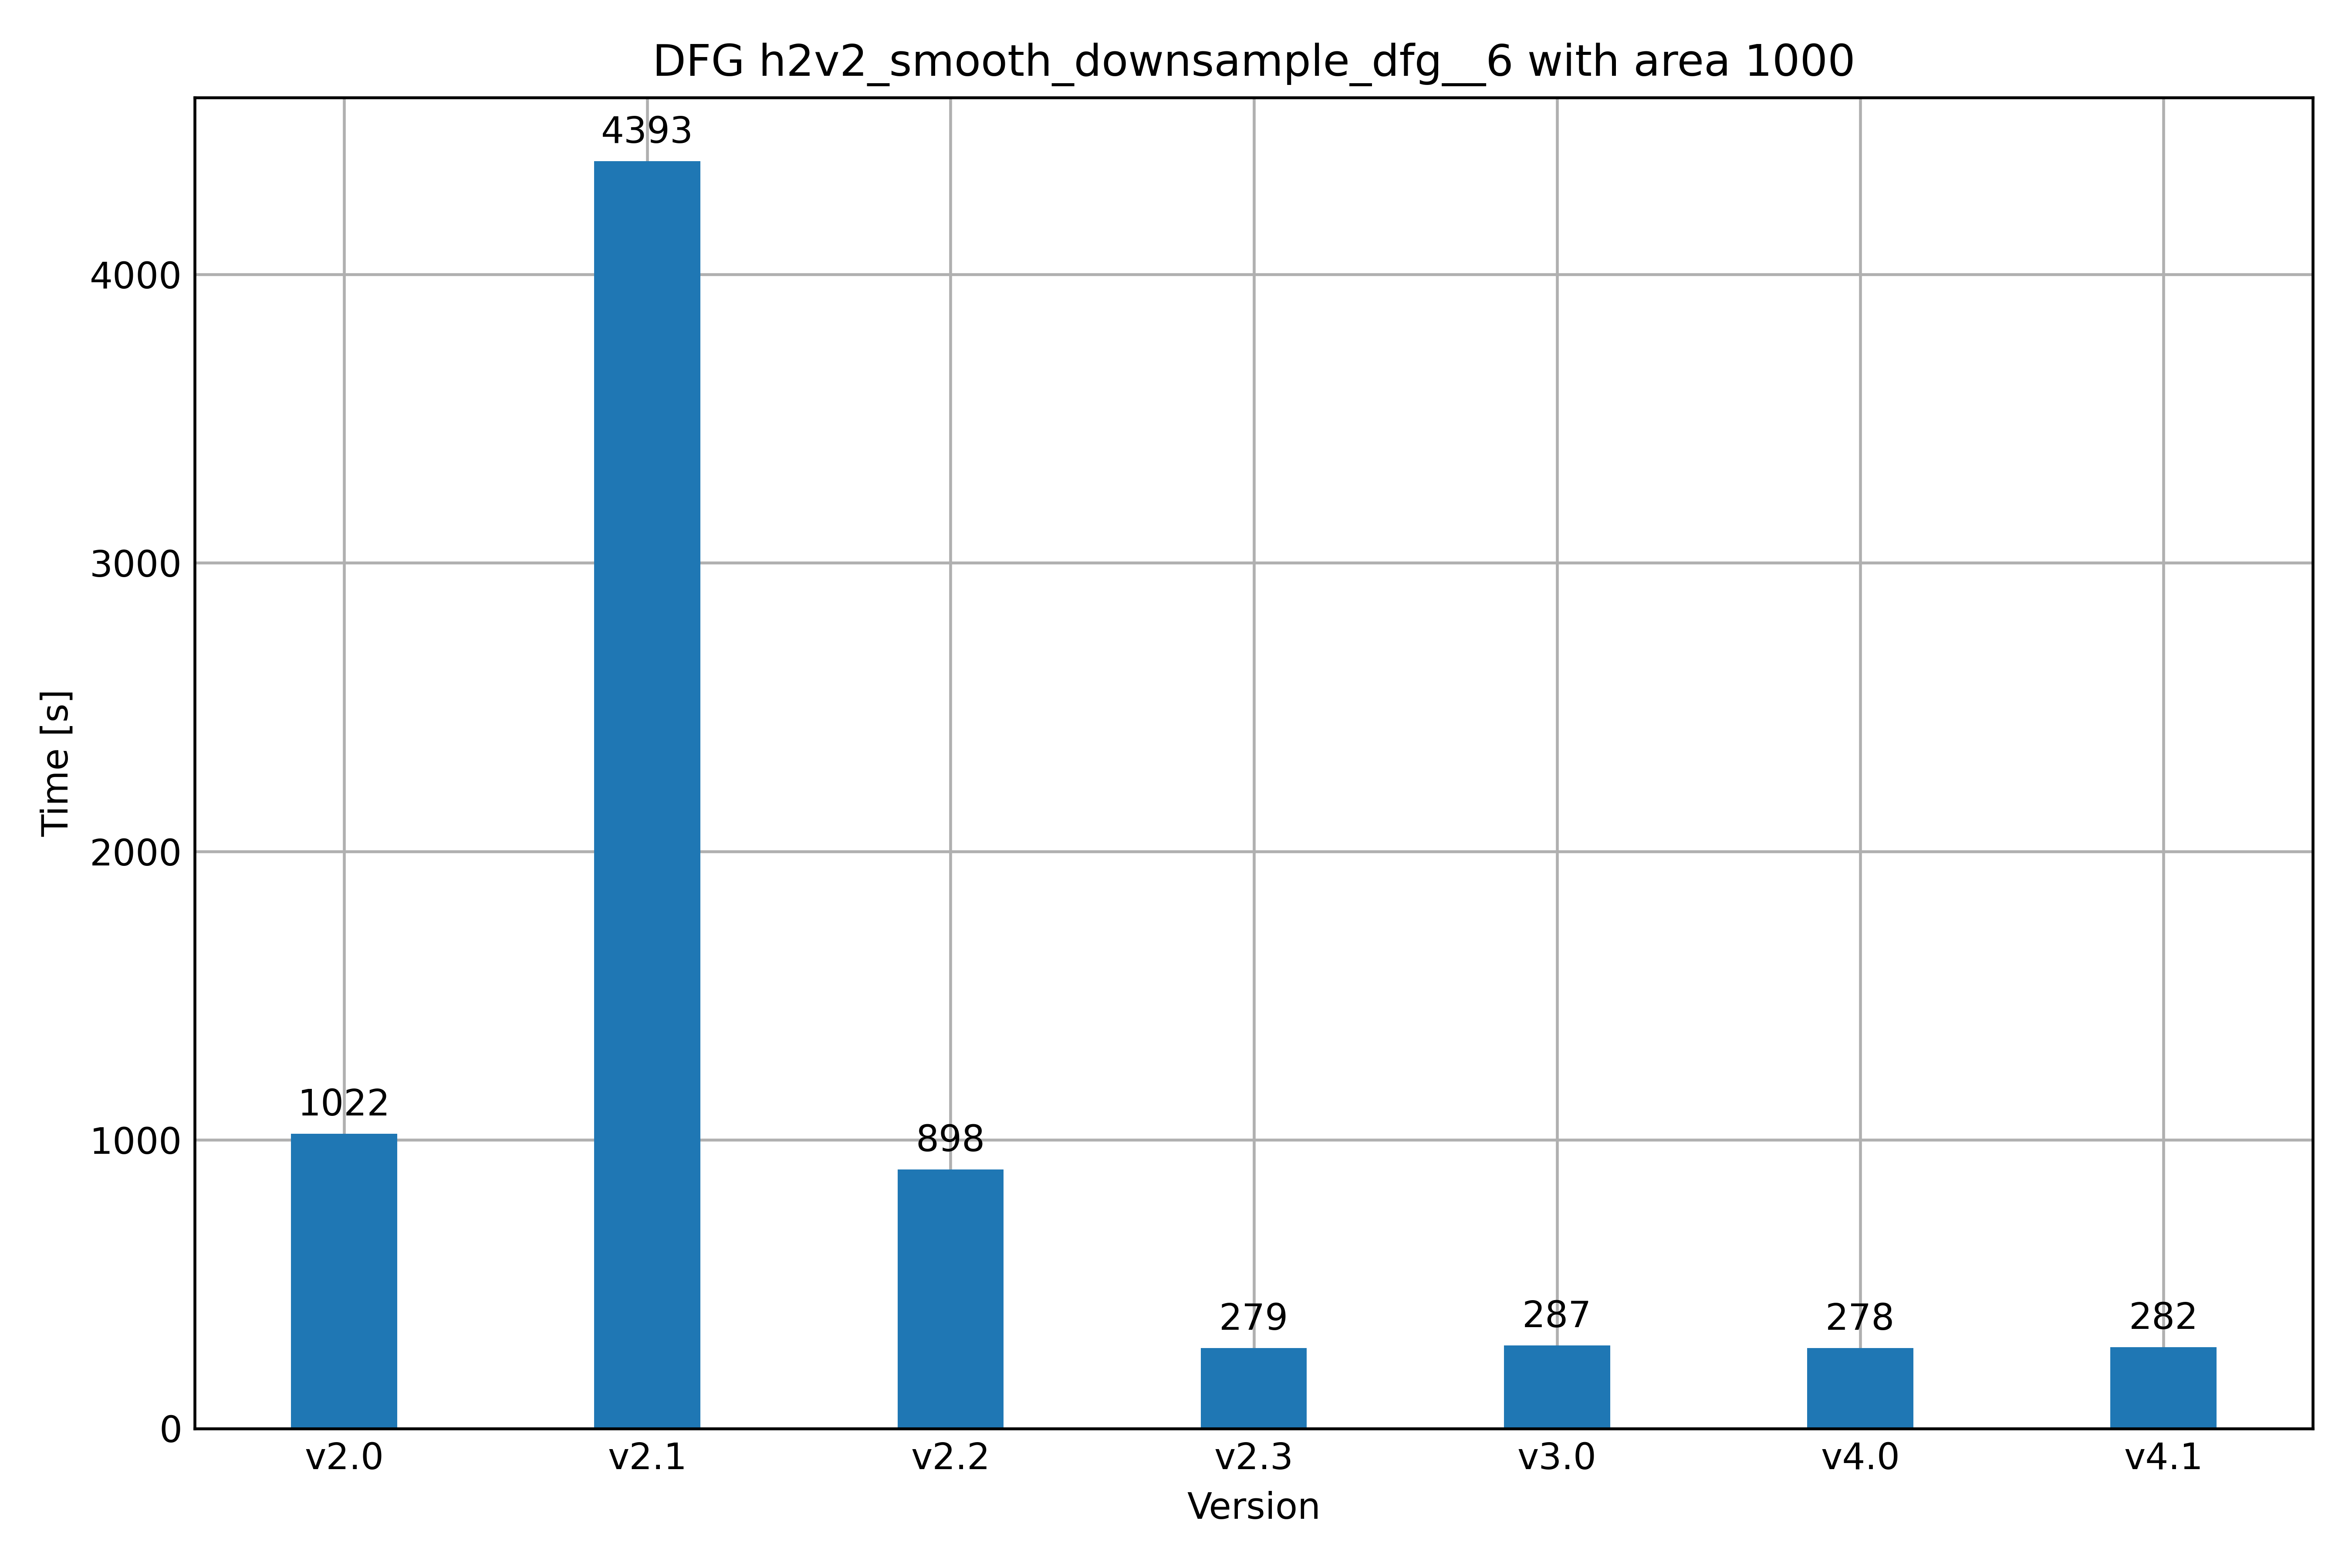
\includegraphics[width=.95\linewidth]{chapters/figures/h2v2_smooth_downsample_dfg__6_1000.png}  
        \caption{h2v2 with area 1000 bar graph}
        \label{fig:h2v2_1000}
    \end{subfigure}
\end{figure}

In the figure \ref{fig:fir_500} and \ref{fig:h2v2_500} it's possible to appreciate the advantage to exploit GPU.
Beside the version 2.1 spent the greatest time, all the others have significant improvement in time, 
also respect to the first basic version 2.0 and 2.3.

Version 2.3, 3.0 and 4.0 have almost the same result, also if 4.0 produces always the best ones. This could be due to 
the virtualization process employed from GPU that, on Jetson Nano, it's quite limited or due to the Operating System internal 
scheduling.

More precise data are available in repository, under \emph{result} folder.

\section{Conclusion}

The code running on GPU respect to the CPU is speed up of 14 times, that is an important quantity.

Like premeditated in chapter \ref{chap3} then last version is the best one. Using the internal registers inside GPU,
the fastest memory type, and using much more blocks inside each stream, has been possible the reach the best performance.

Streams have been important:
\begin{itemize}
    \item they allowed to have a further grade of parallelization of the workload;
    \item they allowed to use asynchronous copy of global memory, much faster than synchronous version, of course this operation 
    have been limitated as much as possible like explained in the above chapters.
\end{itemize}

The final version take care of all possible workload problems is the 4.1 that, cause to this little overhead,
is a little heavier than the 4.0. All the other final version, like 2.3 and 3.0, don't look to have a big 
differences in percentage improvement but, on long execution time, important speed up could be achieved in 4.0 and
the versions 4.1 could be used to handle huge quantity of threads.

% \input{./chapters/chap5}
% \input{./chapters/chap6}
% \input{./chapters/chap_name}
% and so on
%
%%%%%%%%%%%%%%%%%%%%%%%%%%%%%%%%%%%%%%%%%%%%%%%%%%%%%%
%    
% HERE IS WHERE YOU INCLUDE YOUR APPENDICES (IF ANY)
%
\appendix
%%% Appendix A
\chapter{Adder behavioural VHDL}
\label{appendix1}

	\lstinputlisting[language=VHDL, breaklines=true]{appendices/files/adder.vhd}

% \lstinputlisting is an alternative way to import text or code from an external file. In this example the behavioural VHDL description of an adder contained in the file adder.vhd is imported. 
% Note that you can set the language of the code that you want to import (VHDL in this example). When you set the language you will see the keywords of that specific language highlighted in your output pdf file.
%You can set a lot parameters: for some examples take a look at the chapter 'How to document the project' that can you find in DLX_Project.pdf.
%%% Appendix A
\chapter{Elaborate Result}
\label{appendix2}

% and so on
%
%%%%%%%%%%%%%%%%%%%%%%%%%%%%%%%%%%%%%%%%%%%%%%%%%%%%%%
 
\end{document}